\chapter{Modelagem}\label{cap:modelagem}

Neste capítulo é criado um modelo sequencial do problema do futebol de robôs.
Para isso, a arquitetura do futebol de robôs considerada neste trabalho é
detalhada.  São apresentadas definições de termos utilizados nas seções
seguintes, juntamente com um estudo das influências da arquitetura do jogo
descrita anteriormente.

Um modelo abstrato discreto do futebol de robôs é proposto para simplificar o
problema e permitir que sejam feitas várias simulações durante o planejamento
das jogadas.  Também será apresentada a tabela de decisão, necessária para
permitir que o melhor planejamento seja armazenado, bem como incorporar a
mudança de planejamento na função de avaliação.  A função de avaliação utilizada
para avaliar as jogadas.

Devido a complexidade do problema, também foi desenvolvida uma maneira de
incorporar sugestões ao planejamento.  Essas sugestões são chamadas de
\textit{posições chave}, cuja descrição encontra-se no final deste capítulo.

\section{Arquitetura do jogo}\label{sec:arch_ssl}

A arquitetura a ser considerada é baseada em \cite{felixnavarro}.  A
\textit{RoboCup Small Size League} (SSL) envolve vários sistemas.  Logo, com o
objetivo de facilitar a compreensão do problema, a arquitetura do jogo a ser
considerada é apresentada na Figura~\ref{fig:arquitetura_ssl}. Essa arquitetura
é composta pelos seguintes sistema:

\begin{itemize}
  \item Câmeras Visão: conjunto de câmeras \textit{FireWire} que captura as imagens do
        campo e as envia para a SSL-Vision;
  \item Comunicação: módulo responsável por receber os parâmetros
        dos motores, drible, chute baixo e chute alto e enviar o comando via
        ondas de rádio para os robôs;
  \item Mundo Real: campo de futebol real, onde os times 1 e 2 interagem
        através de seus respectivos robôs
  \item Referee-Box: \textit{software} padronizado pela RoboCup para que as
        regras da competição sejam cumpridas sem que haja intervenção
        humana excessiva durante uma partida;
  \item \textit{Software} Time 1/2: \textit{software} do time 1/2;
  \item SSL-Vision: \textit{software} padronizado pela RoboCup que permite a
        integração com um conjunto de câmeras \textit{FireWire} que capturam
        imagens do campo e as processa, extraindo informações de posicionamento
        dos robôs e da bola contidas nessas imagens;
  \item Time 1/2: time de robôs que executa os comandos recebidos pelo
        sistema de transmissão do time 1/2;
  \item Transmissão 1/2: sistema de transmissão do time 1/2;
\end{itemize}

\begin{figure}[thpb]
  \centering
  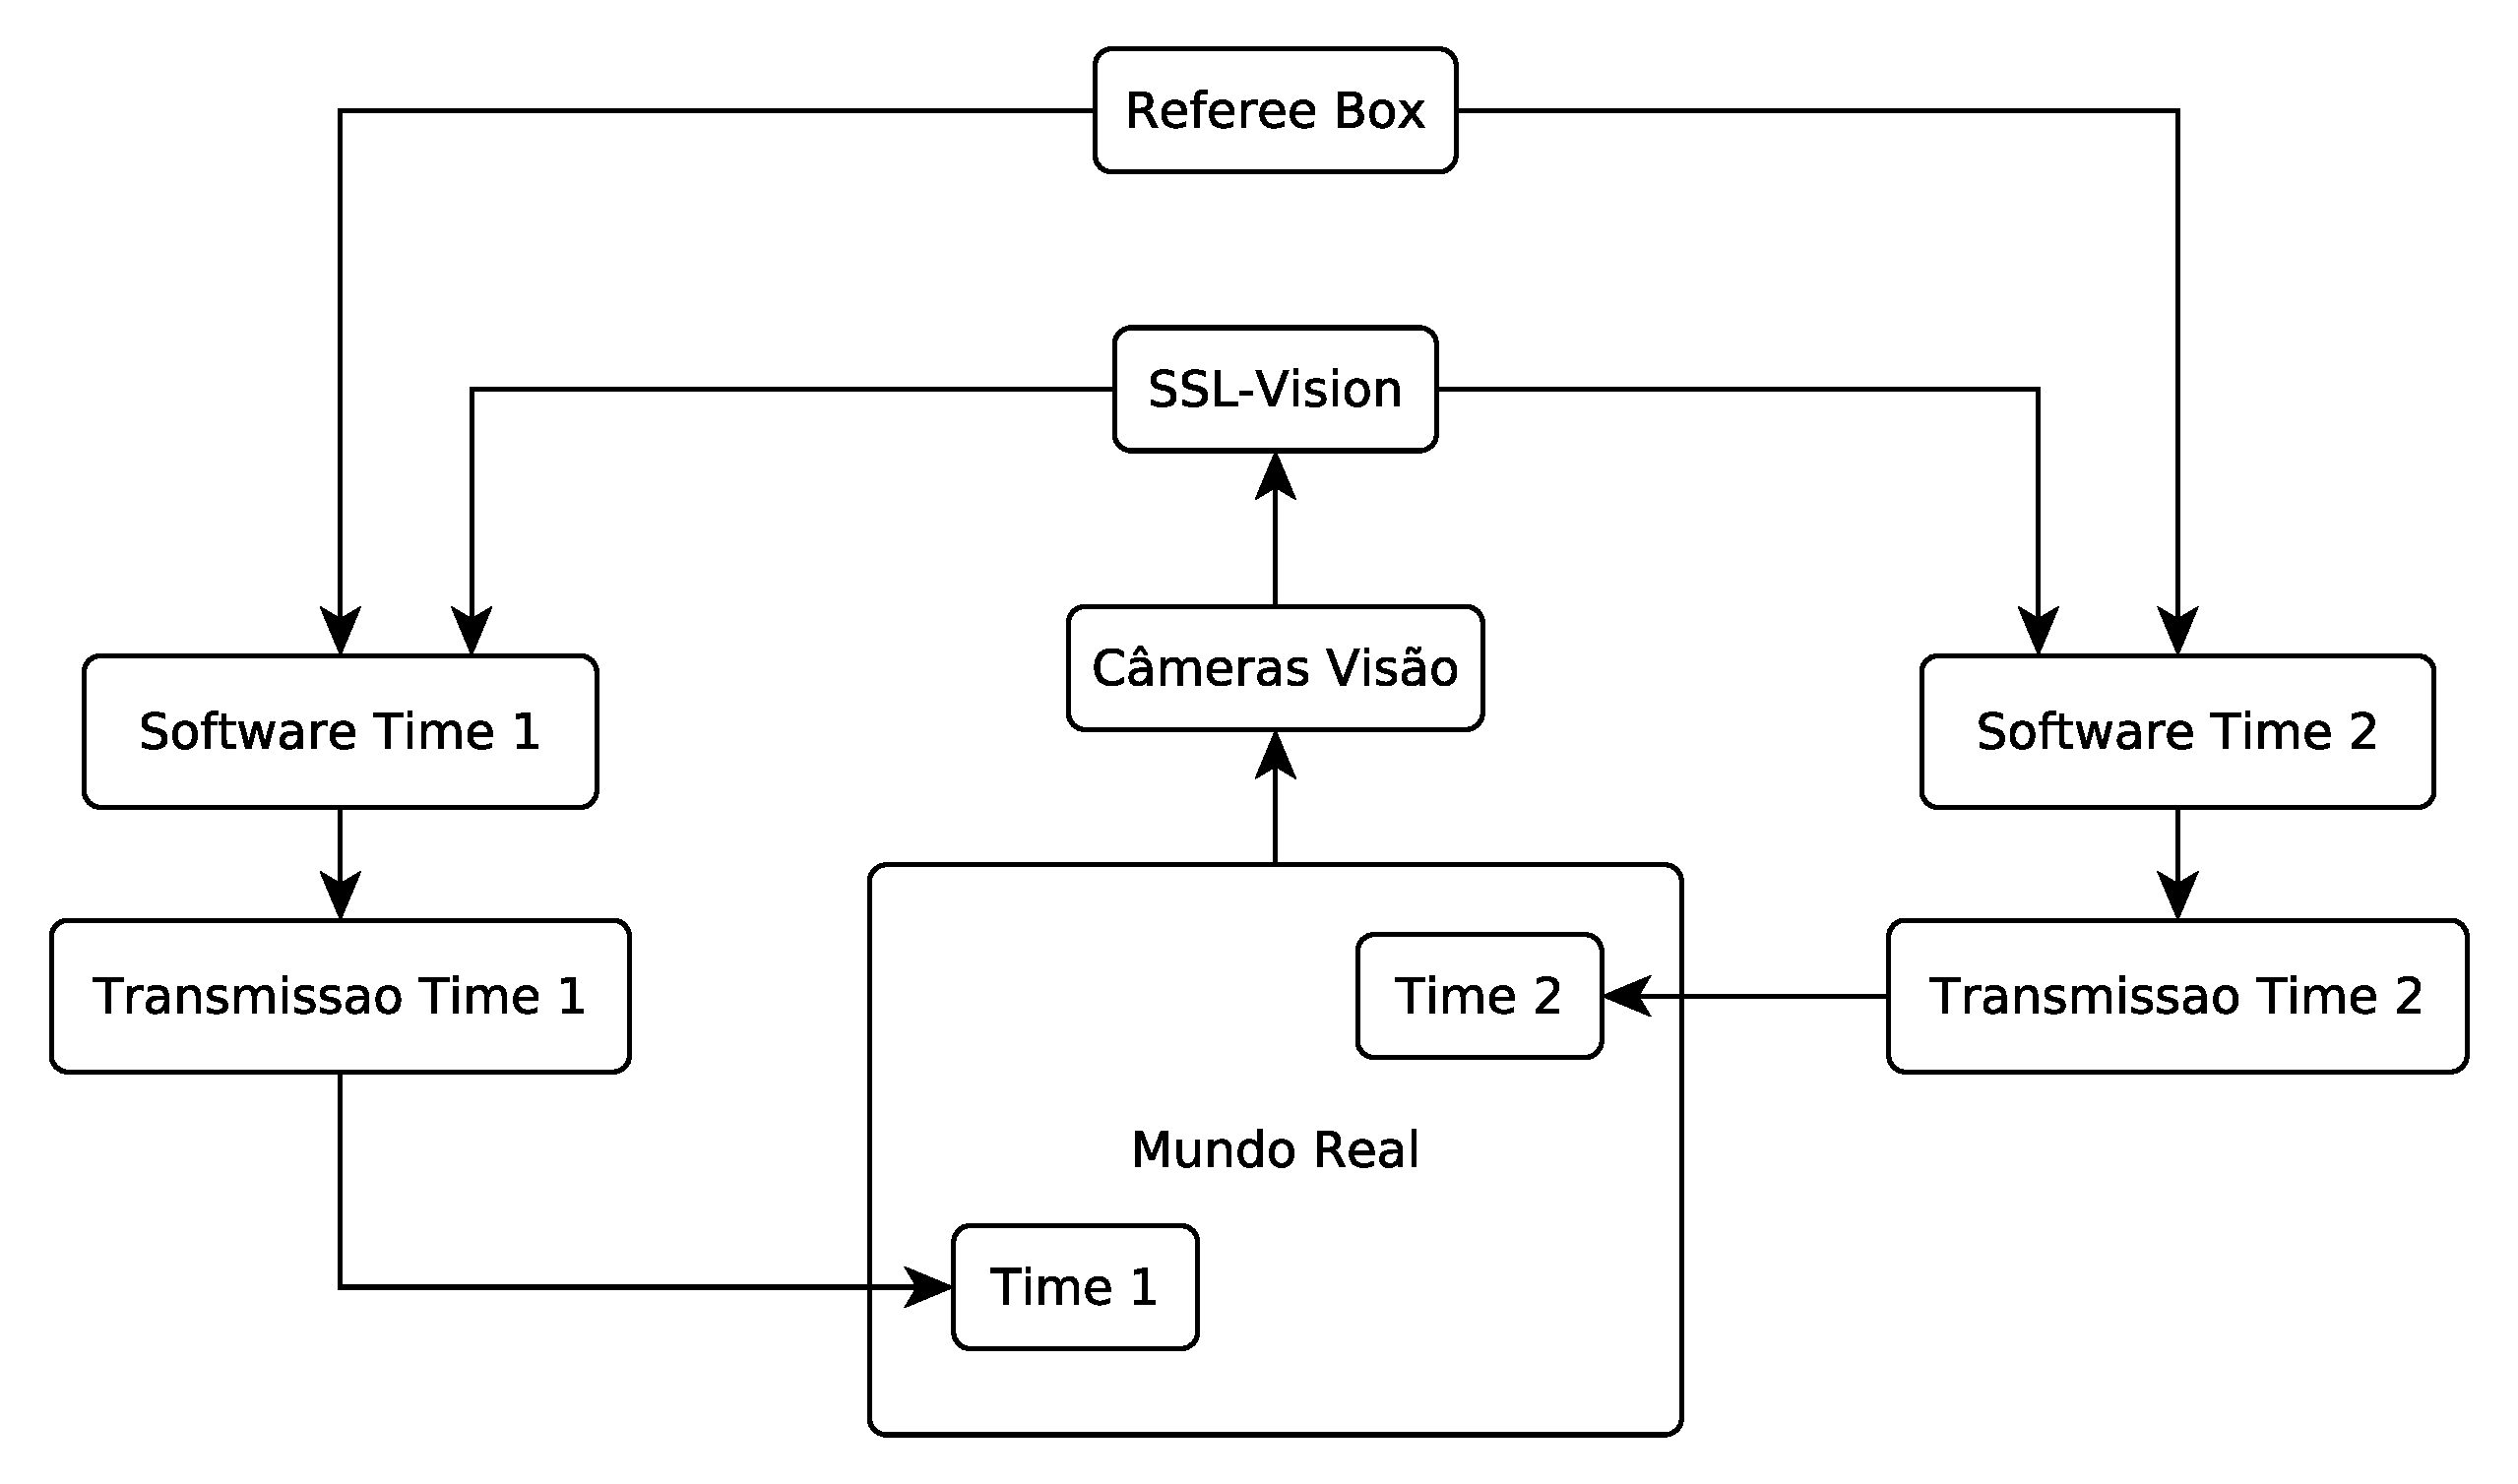
\includegraphics[width= 0.8\linewidth]{img/arq_ssl}
  \caption{Arquitetura básica da SSL}\label{fig:arquitetura_ssl}
\end{figure}

Conforme apresentado na Figura~\ref{fig:robo}, cada robô presente no campo
possui um padrão de cores.  A cor central indica a que time o robô pertence,
podendo ser azul ou amarela.  A disposição das outras cores é utilizada para
identificar o número do robô, i.e., cores diferentes são identificadas com
números diferentes.  A Figura~\ref{fig:padroes_ssl} apresenta os padrões oficias
da competição.

\begin{figure}[thpb]
  \centering
  \includegraphics[width=0.8\linewidth]{padroes_ssl}
  \caption{Padrões oficiais da SSL~\cite{zickler-ssl}}\label{fig:padroes_ssl}
\end{figure}

A posição dos círculos que compõem o padrão são utilizados para calcular a
orientação e posição do robô no campo, conforme ilustrado na
Figura~\ref{fig:rob_data}.  Isso tudo é feito pelo \textit{software} da
SSL-Vision, que se utiliza das imagens capturadas pelas duas câmeras posicionadas
acima do campo.  Esses dados são fornecidos em média a cada $16,6{\ }ms$.  A
Figura~\ref{fig:cmra_campo} mostra a disposição das câmeras no campo.

\begin{figure}[thpb]
  \centering
  \includegraphics[width=0.5\linewidth]{img/rob_data}
  \caption{Parâmetros de estado mutáveis do robô}\label{fig:rob_data}
\end{figure}

\begin{figure}[thpb]
  \centering
  \includegraphics[width= 0.8\linewidth]{img/cmra_campo}
  \caption{Disposição das câmeras no campo}\label{fig:cmra_campo}
\end{figure}

% vim: tw=80 et ts=2 sw=2 sts=2 ft=tex spelllang=pt_br,en

\section{Definições}\label{sec:defs}

\begin{defi}[Corpo Rígido]
  Um corpo rígido $cr$ é definido por dois subconjuntos disjuntos de parâmetros
  $cr= \langle \hat{cr}, \bar{cr} \rangle$ em que:

  \begin{itemize}
    \item $\hat{cr} = \langle pos, \theta, vel, \omega \rangle$, que são os
      parâmetros de estado mutáveis, respectivamente: posição ($\mathbb{R}
      ^{3}$), orientação ($\mathbb{R} ^{3}$), velocidade linear ($\mathbb{R}
      ^{3}$), velocidade angular ($\mathbb{R} ^{3}$)

    \item $\bar{cr} :$ parâmetros imutáveis do corpo que descrevem sua natureza
      fixa e que permanecem constantes ao longo do curso de planejamento.
  \end{itemize}
\end{defi}

Exemplos de parâmetros considerados nesta modelagem imutáveis são: coeficiente
de atrito estático e dinâmico, descrição $3D$ do corpo (por exemplo, por meio de
um conjunto de primitivas $3D$), centro de massa no referencial do corpo,
coeficiente de restituição, coeficiente de amortecimento linear e angular.

\begin{defi}[Bola]\label{def:bola}
  Bola é um corpo rígido $b$, no qual somente as componentes $\langle x,y
  \rangle$ do parâmetro $\hat{b}.pos$ são observáveis.
\end{defi}

De acordo com a arquitetura do jogo descrita na Seção~\ref{sec:arch_ssl}, tem-se
que, a partir de uma sequência de quadros, é possível obter um valor estimado
para o parâmetro $\hat{b}.vel$ a partir do intervalo entre os dados recebidos da
\textit{SSL-Vision} e da equação $ vel \approxeq \frac{\Delta pos}{\Delta t} $.
Entretanto, uma vez que a componente $z$ de $\hat{b}.pos$ não é observável,
$\hat{b}.vel.z$ não pode ser estimada a partir do intervalo entre os dados
recebidos da \textit{SSL-Vision}. Semelhantemente,  uma vez que o parâmetro
$\hat{b}.\theta$ também não pode ser observado, não se pode estimar o valor de
$\hat{b}.\omega$ com exatidão.

% XXX[vbramigk] definir skill

\begin{defi}[Robô]
  Robô, representado por $r$, é um conjunto de sistemas compostos de corpos
  rígidos, \textit{hardware} e \textit{firmware}. Neste trabalho será
  considerado que o robô tem os seguintes sistemas:

  \begin{itemize}
    \item Drible: imprime um torque a bola;
    \item Chute baixo: imprime uma força à bola $b$ e, possivelmente, um torque,
      com o objetivo de alterar as componentes $\langle x,y \rangle$ do
      parâmetro $\hat{b}.vel$;
    \item Chute alto: imprime uma força à bola $b$ e, possivelmente, um torque,
      com o objetivo de alterar as componentes $\langle x,y,z \rangle$ do
      parâmetro $\hat{b}.vel$, com $\hat{b}.vel_z \neq 0$;
    \item Receptor: recebe comandos enviados pelo sistema de transmissão de seu
      respectivo time;
    \item Sistema de movimentação: imprime uma força e um torque ao centro de
      massa global do $r$.
  \end{itemize}
\end{defi}

A Figura~\ref{fig:rob_data} ilustra os parâmetros de estado mutáveis do robô.
Por meio dos sistemas listados acima, cada robô $r$ pode executar um conjunto de
ações $A_{rob}$. A Figura~\ref{fig:robo} apresenta os atuadores típicos de um
robô da SSL.

\begin{figure}[H]
  \centering
  \includegraphics[width=0.8\linewidth]{robo}
  \caption{Atuadores típicos de um robô da SSL}\label{fig:robo}
\end{figure}

Apesar de o modelo descrito acima abranger a maioria dos robôs utilizados
atualmente por equipes da SSL, é importante ressaltar que o robô pode ter um
conjunto de sensores que poderiam coletar informações adicionais às transmitidas
pela \textit{SSL-Vision} juntamente com um sistema de transmissão para enviá-las
ao software do seu respectivo time. Isso é interessante, pois, conforme
observado na Definição~\ref{def:bola}, o parâmetro $\hat{b}.\theta$ não é
observável. Como o sistema de drible impõe um torque à bola, por meio de um
sensor, é possível estimar o valor de $\hat{b}.\omega$. Sem esse sensor, não é
possível prever com exatidão a trajetória da bola somente com informações de
simulação ou da visão.


% TODO: referenciar zicler para exemplos de skills
% TODO: Discrever Skill
%\begin{defi}[Skill]
%  $Sk \subset A_{rob}$ um conjunto de \textit{skills};
%\end{defi}
%
%% TODO: Discrever Tactic
%\begin{defi}[Tactic]
%  $tk = G(V \in Sk, E \in {prob} )$ o conjunto de todas as táticas possíveis
%  formadas a partir de grafos orientados, em que os vértices são \textit{skills} $sk \in Sk$
%  e as arestas são $prob$ associadas a possibilidade de ocorrerem as transições
%  entre uma skill e outra;
%
%% XXX: wtf???
%  $prob: X \longrightarrow [0,1]$ uma distribuição de probabilidade, cujo argumento é
%  $x \in X$;
%\end{defi}
%
%% TODO: Definir agente baseado em utilidade
%\begin{defi}[Tactic]
%  $f_{U}: X \longrightarrow \mathbb{R^{+}} \cup\lbrace 0\rbrace$ uma função utilidade tal que
%  $f_{U}(x)$ reflate a utilidade do estado $x \in X$ um entre estados do mundo dado os estados;
%\end{defi}
%
%% TODO: Definir árvore de busca
%\begin{defi}[Árvore de Busca]
%  $AB =\lbrace V \subset X, E \subset A\rbrace$ uma árvore de busca;
%\end{defi}
%
%% TODO: Definir estratégia (pode ser o BK-BGK)
%\begin{defi}[Estratégia de Busca]
%  $e_b: \langle X_{ob}^{i}, e, f_{U}, r_i, AB\rangle \longrightarrow AB^{'}$ uma estratégia de busca.
%\end{defi}
%
%% TODO: Modelo de reação dos robôs do time adversário
%\begin{defi}[Modelo de reação dos robôs do time]
%  Depende de quão distante no tempo está a reação que se quer
%  estimar. Quanto menor a distância no tempo, mais este modelo
%  se aproxima do modelo dinâmico dos robôs.
%\end{defi}

\begin{defi}[Time]\label{def:time}
  Sejam os seguintes parâmetros:

  \begin{description}
    \item $Rob_c$ o conjunto dos robôs controlados;
    \item $Rob_{ad}$ o conjunto dos robôs adversários, isto é, não controlados;
    \item $X$ o espaço de estado de todos os corpos rígidos envolvidos na partida considerada;
    \item $x_{init} \in X$ o estado inicial;
    \item $X_{goal}\subset X$ o conjunto de estados objetivo;
    \item $x_{ob}^{i}$ os estados observados pelo módulo \textit{SSL-Vision} no instante $i$;
    \item $X_{ob}^{i} =  \lbrace{x_{ob}^{0} = x_{init},\dots,x_{ob}^{i}}\rbrace$;
    \item $Sk \subset A_{rob}$ um conjunto de \textit{skills};
    \item $prob: X \longrightarrow [0,1]$ uma distribuição de probabilidade, cujo argumento é
      $x \in X$;
    \item $tk = G(V \in Sk, E \in {prob} )$ o conjunto de todas as táticas possíveis
      formadas a partir de grafos orientados, em que os vértices são \textit{skills} $sk \in Sk$
      e as arestas são $prob$ associadas a possibilidade de ocorrerem as transições
      entre uma skill e outra;
    \item $A_c = A_{rob 1} \cup \dots \cup A_{rob n_c}$ o conjunto das ações possíveis de $Rob_c$;
    \item $A_{ad} = A_{rob 1} \cup \dots \cup A_{rob n_{ad}}$ o conjunto das ações possíveis de $Rob_{ad}$;
    \item $A = A_c \cup A_{ad}$ o conjunto das ações possíveis de $Rob_c \cup Rob_{ad}$;
    \item $e: \langle x,a \rangle \longrightarrow x^{'}$ a função de transição de estado que pode
      aplicar uma ação $a\in A$ em um estado particular
      $x \in X$ e computar o estado seguinte $x^{'} \in X$;
    \item $f_{U}: X \longrightarrow \mathbb{R^{+}} \cup\lbrace 0\rbrace$ uma função utilidade tal que
      $f_{U}(x)$ mede a utilidade do estado $x \in X$ um entre estados do mundo dado os estados;
    \item $m_{reac{\ }ad}: \langle A_{ad}, X_{ob}^{i}\rangle \longrightarrow a_{ad}^{'}$ o modelo de reação dos robôs
      adversários dado $X_{ob}^{i}$;
    \item $AB =\lbrace V \subset X, E \subset A\rbrace$ uma árvore de busca;
    \item $e_b: \langle X_{ob}^{i}, e, f_{U}, m_{reac{\ }ad}, AB\rangle \longrightarrow AB^{'}$ uma estratégia de busca.
  \end{description}

  Então, um time $T$ é definido por:
  \[
    T: \langle Rob_c, A, X_{ob}^{i}, e, e_b, m_{reac{\ }ad} \rangle \longrightarrow a_c^{i+1}
  \]
\end{defi}

Assim, utilizando-se de $e$, $T$ pode simular várias sequência de ações $a_c$
dado $X_{ob}^{i}$ a partir de $f_{U}$ e $e_b$. Pode-se, a partir de $m_{reac{\
}ad}$, considerar as ações do time adversário baseado em estados anteriores.

% TODO: describe more the notation
\begin{defi}[Partida]
  Dado dois times $T_1$ e $T_2$. Uma partida $p$ é definida por:

  \[
    p = \lbrace T_1, T_2, \Delta t, \delta t, \langle Ref^{0}, X_{ob}^{0}, A_1^{0}, A_2^{0}\rangle, 
    \dots, \langle Ref^{N}, X_{ob}^{N}, A_1^{N}, A_2^{N} \rangle \rbrace
  \]

  Uma sequência, em que:
  \begin{description}
    \item $\Delta t$ é o tempo de duração da partida;
    \item $\delta t$ é o tempo médio entre cada frame enviado pela \textit{SSL-Vision} ao longo de $\Delta t$;
    \item $N \approxeq \frac{\Delta t}{\delta t}$ é número total de frames enviados pela \textit{SSL-Vision}
      ao longo de $\Delta t$;
    \item $Ref^{i}$ são os comandos enviados pelo módulo \textit{Referee-Box} no instante $i$;
    \item $X_{ob}^{i}$ são os dados enviados pelo módulo \textit{SSL-Vision} no instante $i$;
    \item $A_1^{i}$ são as ações executadas por $T_1$ no instante $i$;
    \item $A_2^{i}$ são as ações executadas por $T_2$ no instante $i$.
  \end{description}
\end{defi}

Conforme citado em na Seção~\ref{sec:arch_ssl}, $\delta t$ normalmente é $16,6{\ }ms$.
Um exemplo de $A^{i}$ pode ser visto na Figura~\ref{fig:default_atq}.

\begin{defi}[Logs]
  Dada uma partida $p$. O $log$ de $p$ é definidor por:

  \[
    log(p) = \lbrace p.\langle Ref^{0}, X_{ob}^{0}\rangle, \dots, p.\langle Ref^{N}, X_{ob}^{N}\rangle \rbrace
  \]
\end{defi}

A principal diferença entre uma partida $p$ e $log$ é o desconhecimento das
ações que levaram aos movimentos observados nas partidas. Isso é um metadado
importante quando se quer utilizar os dados de um jogo para aproximar o
comportamento de algum time (i.e., $m_{reac{\ }ad}$).  Este é um problema que
está fora do escopo deste trabalho. Um exemplo de uma abordagem para esse
problema pode ser encontrado em \cite{vail2008crf}.

% vim: tw=80 et ts=2 sw=2 sts=2 ft=tex spelllang=pt_br,en

\section{Discretização do jogo}\label{sec:mapeamento}

% TODO[improvement]: add pictures for better understanding
Uma das dificuldades de se discretizar um sistema é a necessidade de criar uma
abstração válida para o jogo, de modo que o que ocorra na simulação aconteça na
prática caso a mesma situação simulada seja observada no mundo físico.

Essa abstração pode ser separada em duas etapas:

\begin{itemize}
  \item Representação do jogo
  \item Execução do planejamento
\end{itemize}

Essas etapas são descritas a seguir.

\subsection{Representação do jogo}\label{subsec:repres_jogo}

\subsubsection{Posse de bola}

Para simplificar o modelo, foi introduzido o conceito de posse de bola. O robô
que possui a bola é aquele que consegue interceptá-la no menor tempo possível.
Como introduzir um modelo que considere a dinâmica do robô iria introduzir um
custo computacional muito alto, foi utilizado um modelo simplificado. As
simplificações são as seguintes (somente para o cálculo do tempo da
interceptação):

\begin{itemize}
  \item A bola se move a velocidade constante
  \item Os robôs conseguem se mover em uma velocidade máxima
        $\hat{r}.vel_{max}$ em qualquer direção a qualquer momento
\end{itemize}

Dadas essas simplificações, o tempo para atingir o ponto de encontro pode ser
calculado da seguinte maneira:

%  vb.t + pb = vr.t + pr
%  => 0 = (vr^2 - vb^2)t^2 - |pr - pb|^2 - 2.vb.(pb - pr).t
%  => delta = 4.[ (vb.(pb - pr))^2 + (vr^2 - vb^2).|pr - pb|^2]
%  b = -2.vb.(pb - pr) = 2.vb.(pr - pb)
%  b_div_2 = vb.(pr - pb)
%  a = (vr^2 - vb^2)
%  c = -|pr - pb|^2
%  t = -b_div_2 +- sqrt(delta_div_4)
%     -----------------
%            a

\begin{gather}
  \hat{b}.vel \cdot t_{encontro} + \hat{b}.pos = \hat{r}.vel_{max} \cdot t_{encontro} + \hat{r}.pos
\end{gather}

Trabalhando a equação acima, tem-se a seguinte equação do segundo grau:
\begin{gather}  
  0 = (\hat{r}.vel^2_{max}-\hat{b}.vel^2) \cdot t^2 - \parallel \hat{r}.pos - \hat{b}.pos \parallel ^2
     - 2 \cdot \hat{b}.vel \cdot (\hat{b}.pos - \hat{r}.pos) \cdot t_{encontro}
\end{gather}
Logo, tem-se:
\begin{gather}  
  \boxed{t_{encontro} = \frac{ - \hat{b}.vel \cdot (\hat{r}.pos - \hat{b}.pos) \pm \sqrt {\frac{\Delta}{4}}}
                 {(\hat{r}.vel^2_{max} - \hat{b}.vel^2)}}
\end{gather}
Onde $\Delta = 4 \cdot [ ( \hat{b}.vel \cdot (\hat{b}.pos - \hat{r}.pos)) ^2 +
           (\hat{r}.vel_{max}^2 - \hat{b}.vel^2) \cdot \parallel \hat{r}.pos - \hat{b}.pos \parallel ^2]$.

\subsubsection{Ações Consideradas}
% TODO: Citar imagem \ref{fig:robo}
Cada um dos robôs em campo será modelado com as seguintes ações possíveis:
\begin{itemize}
  \item Time no ataque (i.e., com a bola):\\
        $A_{atq} = \lbrace Mover(r_i), Chutar(r_{com{\ }bola}), Passar(r_j,r_{com{\ }bola}):
                    r_i, r_j, r_{com{\ }a{\ }bola} \in Rob_{atq}\rbrace$

  \item Time na defesa (i.e., sem a bola):
        $A_{def} = \lbrace Mover(r_i): r_i \in Rob_{def}\rbrace$
\end{itemize}

% TODO: referenciar ações plan kick and pass do capítulo resultados 
%A Figura~\ref{fig:plan_pass} mostra um planejamento com ações de mover e
%passar. Já a Figura~\ref{fig:plan_kick} mostra um planejamento com uma
%ação de chutar no lugar de passar.

Note que o robô com a bola pode se mover. Entretanto isso é indesejável, já que
a velocidade do passe é maior que a velocidade de movimentação do robô. Também
existe uma restrição quanto à distância máxima que se pode conduzir a bola que,
se não for respeitada, resulta em penalidade para o time do robô infrator.

O nível de complexidade das ações possíveis influi diretamente no número de
ações que poderão ser consideradas a tempo de serem úteis para o jogo real.  Por
exemplo, caso não fosse considerada a ação de passe, esta ação ainda sim poderia
acontecer na prática pela composição de outras ações.  Entretanto, seriam
necessários mais níveis de planejamento, uma vez que ela seria a composição de
chutes e movimentações.  Isso tem a contrapartida de reduzir o número de estados
que podem ser simulados, uma vez que o tabuleiro é dinâmico e o jogo real ser
simultâneo, e não sequencial.  Isso fica mais evidente se fossem utilizadas
somente as \textit{skills} para o planejamento.  A principal desvantagem disso é
que o planejador teria que considerar aspectos como colisões e a orientação dos
robôs no planejamento final.  Além de ser ineficiente, coisas como
posicionamento global dos robôs no campo não teriam estados suficientes na
árvore do jogo para serem úteis.

Outra questão que se deve ter em mente ao se modelar as ações básicas dos robôs
é definir ações muito complexas.  Passando para a linguagem da arquitetura STP
(\textit{Skill, Tactic Play}), se fossem usadas \textit{plays} no lugar de
\textit{tactics}, o espaço de jogadas seria muito limitado e poucas jogadas
seriam geradas pelo computador.  Mais detalhes da arquitetura STP podem ser
encontrados em \cite{browning2004stp}.

Como a complexidade cresce exponencialmente, onde o número de ações básicas é a
base, isso não é um problema que pode ser tratado simplesmente com o aumento da
velocidade de processamento.  Deve-se ajustar o nível de abstração de acordo com
os resultados obtidos nos teste práticos.

\subsection{Execução do planejamento}
% TODO[improvement]: specify add images

Esta etapa do modelo é responsável por converter o resultado do planejamento em
comandos mais concretos.  Conforme evidenciado na seção anterior, é nesta parte
que o planejamento de trajetória deve ser levado em consideração.  Esta é a
parte que leva em consideração o modelo dinâmico do robô.  Como isso é um
problema complexo, com o objetivo de focar o escopo da pesquisa no planejamento
de alto nível, será utilizada a arquitetura de controle do pyroboime.
% Essa parte do sistema será detalhada no Capítulo~\ref{cap:arquitetura}.

% vim: tw=80 et ts=2 sw=2 sts=2 ft=tex spelllang=pt_br,en

\section{Função Objetivo}

A função objetivo $f_U$ é definida pela seguinte expressão:

\begin{dmath}
  f_U = \sum c_i 
\end{dmath}

Onde $\lbrace c_i \rbrace$ é o conjunto formado por custos. Os pesos de cada
custo serão denotados por $p_{descrição}$. São eles:
% TODO: Eu tirei a penalização, mas talvez seja melhor explicar
\begin{enumerate}
  \item Custo da Abertura do Gol
  \item Correção da Abertura do Gol Devido a Movimentação da Bola
  \item Distância Total das Ações $Mover(r)$
  \item Distância Máxima das Ações $Mover(r)$
  \item Mudança do Planejamento da Move Table
  \item Custo do Ataque
  \item Custo das Aberturas vistas por $r \in T_c$
  \item Custo das Aberturas vistas por $r \in T_{ad}$
  \item Custo da Defesa
  \item Número de Receptores
  \item Penalização por Proximidade do Gol do Adversário
  \item Penalização por Proximidade
\end{enumerate}

Além dos parâmetros listados acima, outros parâmetros afetam o comportamento do
time:
\begin{enumerate}
  \item Abertura do gol mínima para chute a gol
  \item Número de ramificações
\end{enumerate}

Esses parâmetros foram os primeiros utilizados no programa.  Ao longo dos testes
realizados, foram criados novos parâmetros.  Entretanto, os parâmetros listados
são suficientes para ilustrar a mudança no comportamento do time.

% OBS: o Maj Duarte circulou o título, mas não sei se foi
%      pelos dois erros de português que tinha aqui...
\subsection{Custo da Abertura do Gol}\label{subsec:custo_gap}

O objetivo deste parâmetro é valorizar as aberturas maiores de acordo com a soma
total das aberturas com relação a cada $r \in T$ e com aberturas maiores.  O
cálculo deste custo é feito da seguinte maneira:

\begin{multline} 
 c_{abertura{\ }gol} = taxa_{abertura{\ }total/max{\ }gol} .
   \sum_{r_i \in T} abertura{\ }gol(bola, r)\\
   + (1 - taxa_{abertura{\ }total/max{\ }gol}) .
   max \lbrace abertura{\ }gol(bola, r): r \in T \rbrace
\end{multline}

As aberturas são calculadas de acordo com a posição de um determinado robô $r$
(obstáculo) e a posição atual da bola. Isso gera um conjunto de segmentos de
reta $\lbrace abertura{\ }gol(bola, r): r \in T \rbrace$.

Este custo afeta diretamente os seguintes custos:
\begin{itemize}
  \item Custo do Ataque
  \item Custo da Defesa
  \item Custo das aberturas do gol vistas por $r\in T_c$
  \item Custo das aberturas do gol vistas por $r\in T_{ad}$
\end{itemize}

\subsection{Correção da Abertura do Gol Devido a Movimentação da Bola}

O objetivo deste parâmetro é incorporar a movimentação da bola pelo atacante no
cálculo da abertura do gol. Isso é importante, pois defensores mais próximos são
mais facilmente driblados que defensores mais distantes. Isso pode ser
visualizado na figura \ref{fig:kick_pos}, onde foi considerada uma variação de
15cm e de 0cm. Essa variação é medida na linha normal à reta formada pela bola e
pelo robô em questão.

% TODO: Adicionar gráfico detalhado as contas
%       vide arquivo board.cpp para detalhes de implementação

\begin{figure}[H]
  \centering
  \includegraphics[height=0.4\linewidth]{kick_pos_var_1}
  \includegraphics[height=0.4\linewidth]{kick_pos_var_2}
  \caption{Abertura do gol considerando-se uma variação de 15cm na posição da
  bola (esquerda) e sem variação (direita)}\label{fig:kick_pos}
\end{figure}


\subsection{Distância Total das Ações $Mover(r)$}

O objetivo deste parâmetro é valorar o custo da mudança de estado na função
objetivo. Ele é formado pela soma das distâncias que cada ação $Mover(r)$ irá
percorrer partindo das respectivas posições do estado atual.

\begin{dmath}
 c_{dist{\ }total{\ }mover} = p_{dist{\ }total{\ }mover} .
 \sum_{r_i \in T_c} \lVert pos_{r_i} - Mover(r_i)\rVert
\end{dmath}

\subsection{Distância Máxima das Ações $Mover(r)$}

O objetivo deste parâmetro é incorporar o custo da mudança de estado na função
objetivo. Ele é formado pela ação $Mover(r)$ do planejamento atual com maior
deslocamento.

\begin{gather}
 c_{dist{\ }max{\ }mover}= p_{dist{\ }max{\ }mover} .
 max \lbrace r_i \in T_c : \lVert pos_{r_i} - Mover(r_i)\rVert \rbrace
\end{gather}

\subsection{Mudança do Planejamento da Tabela de Decisão}\label{subsec:change_cost}

O objetivo deste parâmetro é evitar mudanças grandes no planejamento da ação
$Mover(r)$. Uma das razões para isso é evitar um modelo dinâmico exato neste
nível de planejamento, já que isso aumentaria muito o custo computacional desta
etapa do planejamento e, consequentemente, reduziria o número de simulações
possíveis. Por essas razões mudanças no planejamento das ações $Mover(r)$
inicialmente foram penalizadas de acordo com a distância euclidiana entre o
$Mover_p(r)$ planejado anteriormente e o $Mover_{m}(r)$ modificado, conforme a
equação:

\begin{dmath}
 c_{mudança{\ }mover} = p_{mudança{\ }mover} .
 max \lbrace \sum_{r_i \in T_c} \lVert Mover(r_i) - Mover_p(r_i)\rVert \rbrace
\end{dmath}

Isso permite que sejam selecionados $Mover_{m}(r)$ mais próximos do
$Mover_p(r)$, refinado assim o planejamento anterior. Entretanto, um parâmetro
mais significativo é o valor absoluto do ângulo entre essas ações e a posição de
$r$, $\lVert ang(r, Mover_{m}(r), Mover_p(r)) \rVert$.  Dessa maneira, tem-se
que este custo é computado da seguinte maneira:

\begin{dmath}
 c_{mudança{\ }mover} = p_{mudança{\ }mover} .
 max \lbrace \sum_{r_i \in T_c} \lVert ang(r, Mover_{m}(r), Mover_p(r)) \rVert \rbrace
\end{dmath}

\subsection{Custo do Ataque}

Este custo valoriza situações nas quais o time em questão possui o domínio da
bola (descrito na Subsecção~\ref{subsec:repres_jogo}).

\begin{dmath}
 c_{ataque} = p_{ataque} . abertura{\ }gol_{ad}
\end{dmath}

Onde $abertura{\ }gol_{ad}$ é o valor da abertura do gol adversário visto pelo
robô que tem domínio da bola.

\subsection{Custo da Defesa}

Quando não se tem o domínio da bola a abertura do gol do time em questão visto
pelo robô do time adversário que tem a bola é utilizado como penalização
adicional.

\begin{dmath}
  c_{defesa} = p_{defesa} .
   \sum_{r_i \in T_ad} abertura{\ }gol_c(r_i)
\end{dmath}

\subsection{Custo das Aberturas do Gol Vistas por $r\in T_c$}

Este custo tem o objetivo de valorizar configurações nas quais os robôs que não
tem a bola possuam visada para o gol do time adversário.  Isso é desejável, já
que permite que um gol seja feito caso o robô que esta com a posse de bola
execute um passe para um dos robôs em questão.

\begin{dmath}
   c_{abertura{\ }gol{\ }ad} = p_{abertura{\ }gol_{ad}} .
    \sum_{r_i \in T_c} abertura{\ }gol_{ad}(r_i)
\end{dmath}

\subsection{Custo das Aberturas do Gol Vistas por $r\in T_{ad}$}

Este custo é o análogo do custo anterior, mas para o time adversário. Ele visa
penalizar situações nas quais os robôs adversários tenham grande visada (i.e.,
abertura) para o gol.

\begin{dmath}
   c_{bloqueio{\ }gol} = - p_{bloqueio{\ }gol} .
    \sum_{r_i \in T_{ad}} abertura{\ }gol_{ad}(r_i)
\end{dmath}

\subsection{Número de Receptores}

Este custo visa valorizar situações nas quais existam vários robôs que possam
receber passe.

\begin{dmath}
  c_{receptores} = p_{receptores} .
   num \lbrace r_{receptor_i} \rbrace
\end{dmath}

\subsection{Penalização por Proximidade do Gol do Adversário}

Esta penalização visa evitar que os robôs que estão no ataque se concentrem
dentro da área do time adversário. Caso este parâmetro não seja adicionado, é
esse o comportamento resultante do custo das aberturas vistas pelos robôs do
time em questão.  A partir de uma determinada distância, é adicionada uma
parcela de penalização na função objetivo.

\begin{dmath}
  c_{penalização{\ }prox} = - p_{penalização{\ }prox}
    \sum num \lbrace r_{perto} \rbrace
\end{dmath}

\subsection{Abertura Mínima para Chute a Gol}

Este parâmetro é o ângulo total da abertura do gol para permitir o chute pelo
atacante. Ele é relevante, pois afeta o comportamento do atacante e, como
consequência, o comportamento do time durante a posse de bola. Quando a abertura
do gol é menor que este valor, o atacante tem ação de chutar em direção ao goal.

% TODO: Adicionar imagem para ilustrar este caso, já que não tem
%       equações envolvidas

\subsection{Número da Ramificação}

Este parâmetro é o número de possibilidades que serão simulados em cada iteração
do algorítimo de avaliação. Ele influencia o tempo de resposta do planejamento.

% vim: tw=80 et ts=2 sw=2 sts=2 ft=tex spelllang=pt_br,en

\section{Estratégia de Busca}\label{sec:est_busca}
A estratégia de busca utilizada para gerar os novos
estados a partir do estado atual $x$ é apresentada na
Figura~\ref{fig:estr_busca}.

\begin{figure}[H]
  \centering
  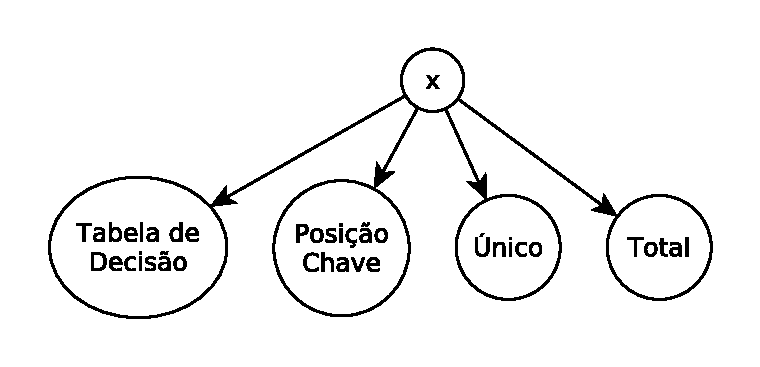
\includegraphics[width= 0.8\linewidth]{tab_dec}
  \caption{Ilustração da distribuição dos tabuleiros
           considerados no planejamento}\label{fig:estr_busca}
\end{figure}

Os tipos de ações que são geradas são:
\begin{itemize}
  \item \textit{Tabela de decisão}: Ação escolhida no último planejamento
  \item \textit{Único}: Ação gerada a partir da tabela de decisão
        onde a ação de um único robô foi modificada
  \item \textit{Total}: Ação gerada a partir da tabela de decisão
        onde a ação do time completo foi modificada
  \item \textit{Posição Chave}: Ação gerada utilizando posições chave
        (vide Seção~\ref{subsec:pos_chave})
\end{itemize}

A ação selecionada é aquela que gera o maior valor de $f_U$.

\subsection{Distribuição da Ação $Mover(r)$}\label{subsec:distr_mov}

Para gerar as ações do tipo $Mover(r)$, são utilizadas três distribuições
uniformes circulares. Essas distribuições tem centro na posição $r.pos$.
São utilizadas para concentrar localmente as movimentações de cada robô.

% vim: tw=80 et ts=2 sw=2 sts=2 ft=tex spelllang=pt_br,en

\subsection{Tabela de Decisão}\label{sec:tab_dec}
A tabela de decisão contém a memória das últimas
decisões $a_{old} \in A_c$ de todos os robôs de $T_c$.
Isso é incorporado ná próxima rodada do algorítmo,
conforme ilustrado na figura~\ref{fig:estr_busca}.


Devido a movimentação dos robôs em $Rob_{ad}$, somente as
ações $Mover(r_i)$ e $Chutar(r_{com{\ }bola})$ são guardadas
intergralmente. No caso da ação $Passar(r_j, r_{com{\ }bola})$,
devido a restrição de o robô que recebe interceptar a bola
antes dos robôs em $Rob_{ad}$, o calculo do receptor $r_j$ é
feito a cada rodada. O receptor anterior só entra no custo
da mudança (vide secção~\ref{subsec:change_cost}). 

Caso a posse de pola passe para o time adversário, o robô
que possuia a bola anteriormente fica com a sua última
ação do tipo $Mover(r_i)$.

\section{Posições Chave}
% TODO
em produção


% vim: tw=80 et ts=2 sw=2 sts=2 ft=tex


% Ramificação constante ou taxa constante

% vim: tw=80 et ts=2 sw=2 sts=2 ft=tex spelllang=pt_br,en
